\documentclass[10pt,a4paper,landscape]{article}
\usepackage[headheight=14pt,left=0.55cm,right=0.55cm,top=1.10cm,bottom=0.55cm,landscape,
headsep=2mm]{geometry}

\usepackage{lastpage}
\usepackage{fancyhdr}
\usepackage{multicol}
\usepackage[utf8]{inputenc}
\usepackage[german]{babel}
\usepackage{graphicx}
\usepackage{wrapfig}
\usepackage{enumitem}
\usepackage{titlesec}
\usepackage{tabularx}
\usepackage[T1]{fontenc}
\usepackage{lmodern}
\usepackage{todonotes}
\usepackage{amsmath}
\usepackage{amssymb}
%\usepackage{showframe}


% Header
\pagestyle{fancy}
\fancyhead{}
\fancyfoot{}
\fancyhead[L]{Zusammenfassung Algorithmische Graphentheorie WiSe 2019/2020}
\fancyhead[R]{Seite $\thepage$ von $\pageref{LastPage}$}
\fancyheadoffset{0cm}

% Document
\setlength{\columnseprule}{0.5pt}
\setlength{\topskip}{10pt}
%\setlist{nosep}

% \titleformat*{\section}{\normalsize\bfseries}
% \titleformat*{\subsection}{\small\bfseries}
% \titleformat*{\subsubsection}{\small\bfseries}
% \titleformat*{\subsubsection}{\bfseries}
% \titleformat*{\subsubsubsection}{\bfseries}

\titlespacing*{\section}
{0pt}{0pt}{0pt}
\titlespacing*{\subsection}
{0pt}{10pt}{0pt}
\titlespacing*{\subsubsection}
{0pt}{5pt}{0pt}

\newcolumntype{P}[1]{>{\centering\arraybackslash}p{#1}}
\newcolumntype{M}[1]{>{\centering\arraybackslash}m{#1}}

\makeatletter
\newcommand{\xRightarrow}[2][]{\ext@arrow 0359\Rightarrowfill@{#1}{#2}}
\makeatother

% Building blocks
\newcommand{\heading}[1]{\noindent\section*{\framebox[\columnwidth][l]{#1}}}
\newcommand{\subheading}[1]{\noindent\subsection*{\framebox[\columnwidth][l]{#1}}}
\newcommand{\subsubheading}[1]{\noindent\framebox[\columnwidth][l]{#1}}
\newcommand{\ccontent}[1]{\parbox{\columnwidth}{\centering{#1}}}

\newenvironment{allesInCode}{\ttfamily}{\par}


% Content
\title{ Algorithmische Graphentheorie }
\author{ Ismael Agchar }
\date{\today}

\begin{document}

% \maketitle
% \newpage
\tableofcontents
\newpage

\begin{multicols*}{2}
\normalsize
\section{ Grundlagen }
    \subsection{ Graphen und Digraphen }
    
    \subsubsection*{ Graph $G$ }  
    \[ G = (V,E) \]
    wobei $V$ eine endliche, nichtleere Menge an Knoten oder Ecken (Vertices) und $E$ eine Menge Kanten (Edges) 
    , gegeben durch ungeordnete Paare von Knoten $(v,w) v, w \in V$, ist.
    
    \subsubsection*{ Digraph $D$ }
    \[ D = (V,A)\]
    wobei $V$ eine endliche, nichtleere Menge an Knoten oder Ecken (Vertices) und $A$ eine Menge von gerichteten 
    Bögen (Arcs) $A \subseteq V \times V$ mit Gewichten $c \in \mathbb{R}$. Ein Digraph heißt konservativ, wenn er 
    keinen Kreis mit negativem Gesamtgewicht enthält.

    \subsubsection*{ Grad eines Knotens $v$ }
    $deg(v) :=$ Grad von v - Anzahl zu Knoten $v$ inzidenter (benachbarter) Kanten in einem Graphen \\
    $deg_{+}(v), deg_{in}(v) :=$ Eingangsgrad von $v$ - Anzahl aller auf $v$ zeigenden Bögen in einem Digraphen \\
    $deg_{-}(v), deg_{out}(v) :=$ Ausgangsgrad von $v$ - Anzahl aller von $v$ ausgehenden Bögen in einem Digraphen 

    \subsubsection*{ Kantenzug/Kette/Pfad $P$ }
    \[ P = (v_0, e_1, v_1, e_2, v_2, \dots, e_k, v_k), v_i \in V, e_i \in E \]
    ist eine Sequenz zusammenhängender Kanten. 
    \subsubsection*{ Weg } ist ein Kantenzug, bei dem alle Kanten (paarweise) verschieden sind, also keine wiederholt wird.
    \subsubsection*{ Kreis/Zyklus } ist ein geschlossener Weg mit identischem Start und Zielknoten.

    \subsubsection*{ vollständiger Graph $K_{n}$ } ist der Graph aus $n$ Knoten, der jeden Knoten mit jedem anderen Knoten verbindet.
    \subsubsection*{ bipartiter Graph } Die Knotenmenge $V$ kann in zwei disjunkte Teilmengen $V_1$ und $V_2$ aufgeteilt werden, sodass jede Kante einen 
    Endpunkt in $V_1$ und $V_2$ hat.
    \subsubsection*{ Satz von König }
    Ein Graph ist genau dann bipartit, wenn er keinen Kreis ungerader Länge enthält.

    \subsection{ Bäume und Wälder }
    \subsubsection*{ Wald $F$ } ist ein Graph, der keinen Kreis enthält.
    \subsubsection*{ Baum $T$ in einem Graphen $G$ } ist ein zusammenhängender Wald. $T$ heißt aufspannend, wenn er alle Knoten von $G$ enthält. 

    \subsection{ Handshaking-Lemma }
    In einem Graphen $G = (V, E)$ gilt:
    \[ \sum_{v\in V} deg(v) = 2|E| \]
    Daraus folgt implizit, dass die Anzahl der Knoten mit ungeradem Grad gerade ist.

    \subsection{ Planare Graphen }
    Ein planarer Graph kann auf einer zweidimensionalen Fläche kreuzungsfrei gezeichnet werden. Jeder Kreis, 
    jeder Baum und der vollständige Graph $K_4$ sind planar. Der vollständige Graph $K_5$ und der vollständige 
    bipartite Graph $K_{3,3}$ sind nicht planar.
    \subsubsection*{ Satz von Kurtowski } ein Graph ist genau dann nicht planar, wenn er durch Kontraktion von Kanten 
    in den $K_5$ oder den $K_{3,3}$ überführt werden kann.
    \subsubsection*{ Eulersche Polyederformel }
    \[ n - m + f = 2 \]
    wobei $n$ die Anzahl der Knoten, $m$ die Anzahl der Kanten und $f$ die Anzahl der Flächen in einem 
    zusammenhängenden planaren Graphen ist. \\
    Für nicht zusammenhängende Graphen gilt
    \[ n - m + f = k + 1 \]
    wobei $k$ die Anzahl der Zusammenhangskomponenten ist. \\
    Aus der Polyederformel folgt unmittelbar für planare Graphen aus 3 oder mehr Knoten:
    \[ m \leq 3n - 6 \]
    \[ f \leq 2n - 4 \]
    Ist der Graph außerdem noch bipartit gilt für die Anzahl der Kanten:
    \[ m \leq 2n - 4 \]
    Insbesondere hat jeder planare Graph mindestens einen Knoten von Grad höchstens 5.

    \subsection{ Topologische Sortierung }
    Eine topologische Sortierung eines Digraphen $D = (V,A)$ ist eine injektive Abbildung 
    $f:V\Rightarrow \mathbb{N}$, sodass gilt:
    \[ (v,w)\in A \Rightarrow f(v) < f(w) \]
    Ein Digraph hat genau dann eine topologische Sortierung, wenn er keinen gerichteten Kreis enthält.
    \newpage
    \subsubsection*{ TopSort }
    \small
\begin{verbatim}
input:  ein beliebiger Digraph
output: eine topologische Sortierung, gegeben durch die 
        Knoten-Index-Beziehung oder die Aussage, dass ein Kreis vorliegt

index = 0
sort()

while( es ist ein Knoten v mit Eingangsgrad > 0 vorhanden )
    entferne v und aktualisiere die Eingangsgrade seiner Nachbarn
    sort(v) = index
    index++

if( es sind noch Knoten übrig )
    return false, es liegt ein Kreis vor
else 
    return sort
    \end{verbatim}
\normalsize

\section{ Suche in Graphen }
    Suchverfahren für Graphen traversieren alle von einem Startknoten $s$ aus erreichbaren Knoten 
    eines Graphen $G = (V,E)$ nach einem rekursiven Schema. Jedem traversierten Knoten wird sein Index 
    (Reihenfolge der Traversierung), sein Vorgänger und sein Abstand zum Startknoten $s$ zugeordnet.
    Aus den Vorgänger-Beziehungen lässt sich ein aufspannender Baum von $G$ mit Wurzel $s$ rekonstruieren.
    \newline
    Außerdem gilt für die Breitensuche: ein zusammenhängender Graph ist genau dann bipartit, wenn es bei der Breitensuche mit beliebigem Startknoten 
    keine Nicht-Baumkante $e$ gibt, die eine Querverbindung im Spannbaum darstellt ($e$ verbindet zwei Baumknoten 
    auf gleicher Höhe des Baumes).
    \subsection{ Breitensuche (BFS) }
    \small
\begin{verbatim}
input:  ein zusammenhängender Graph G, 
        ein Startknoten s
output: Index der Traversierung, Vorgänger und Abstand von s für 
        jeden von s aus erreichbaren Knoten

counter = 1
index()
distance()
predecessor()
queue

foreach( Knoten v von G )
    if( v = s )
        index(v) = 1
        distance(v) = 0
        predecessor(v) = undefined
        füge v in queue ein
    else
        index(v) = undefined
        distance(v) = undefined
        predecessor(v) = undefined

while( queue ist nicht leer )
    v = head(queue)
    if( v hat einen noch nicht untersuchten Nachbarn w )
        markiere w als untersucht
        füge w am Ende der queue ein
        index(w) = ++counter
        predecessor(w) = v
        distance(w) = distance(v) + 1
    else
        entferne v aus der queue

return index, predecessor, distance
    \end{verbatim}
\normalsize
    
    \subsection{ Tiefensuche (DFS) }
    \small
\begin{verbatim}
input:  ein zusammenhängender Graph G, ein Startknoten s
output: Index der Traversierung, Vorgänger und Abstand von s für 
    jeden von s aus erreichbaren Knoten

counter = 1
index()
distance()
predecessor()
stack

foreach( Knoten v von G )
    if( v = s )
        index(v) = 1
        distance(v) = 0
        predecessor(v) = undefined
        lege v auf stack
    else
        index(v) = undefined
        distance(v) = undefined
        predecessor(v) = undefined

while( stack ist nicht leer )
    v = peek(stack)
    if( v hat einen noch nicht untersuchten Nachbarn w )
        markiere w als untersucht
        lege w auf stack
        index(w) = ++counter
        predecessor(w) = v
        distance(w) = distance(v) + 1
    else
        nimm v von stack

return index, predecessor, distance
    \end{verbatim}
\normalsize


\section{ Minimal aufspannende Bäume }
    Ein minimal aufspannender Baum, ist der aufspannende Baum, mit der kleinsten Gesamtsumme der Kantengewichte.
    Jeder aufspannende Baum mit $n$ Knoten hat genau $n-1$ Kanten. Entfernt man eine Kante $e$, ist der 
    aufspannende Baum nicht mehr zusammenhängend, sondern in zwei Zusammenhangskomponenten zerlegt - den zu $e$ 
    gehörigen Fundamentalschnitt. Fügt man dem aufspannenden Baum eine Kante $k$ hinzu, enthält der Baum nun 
    einen Kreis - den zu $k$ gehörigen Fundamentalkreis.
    \subsection{ Kruskal }
    \small
\begin{verbatim}
input:  ein zusammenhängender Graph mit Kantengewichten
output: ein minimal aufspannender Baum

sortiere alle Kanten aufsteigend nach ihren Gewichten
counter = 0
tree

initialisiere für jeden Knoten v eine Zusammenhangskomponente V, 
die nur v enthält

foreach( Kante e der aufsteigend sortierten Kanten )
    if( e verbindet zwei unterschiedliche Komponenten V und W )
        verschmilz V und W
        füge e zu tree hinzu
        counter++
        if( counter = Anzahl aller Knoten - 1 )
            return tree
    \end{verbatim}
\normalsize

    \subsection{ Prim }
    \small
\begin{verbatim}
input:  ein zusammenhängender Graph mit Kantengewichten, 
        ein Startknoten s
output: ein minimal aufspannender Baum gegeben durch eine 
        Vorgänger-Beziehung

predecessor()
distance()

foreach( Knoten v des Graphen )
    predecessor(v) = undefined
    if( v = s )
        distance(v) = 0
    else
        distance(v) = infinity

while( noch nicht alle Knoten erreichbar )
    v = noch nicht erreichbarer Knoten mit minimalem dist(v)
    foreach( noch nicht erreichbarer Nachbar w von v )
        if( distance(w) > Kantengewicht(v,w) )
            distance(w) = Kantengewicht(v,w)
            predecessor(w) = v
    markiere v als erreichbar
    \end{verbatim}
\normalsize


\section{ Kürzeste Wege }
    \subsection{ Dijkstra }
    \small
\begin{verbatim}
input:  ein gewichteter Digraph mit nichtnegativen Kantengewichten,
        ein Startknoten s
output: die kürzesten Wege von s zu jedem anderen erreichbaren Knoten, 
        gegeben durch eine Vorgänger Beziehung,
        die absoluten Distanzen von s zu jedem anderen Knoten

predecessor()
distance()

foreach( Knoten v des Graphen )
    predecessor(v) = undefined
    if( v = s )
        distance(v) = 0
    else
        distance(v) = infinity

while( es gibt nicht markierte Knoten v mit distance(v) < infinity )
    v = nicht markierter Knoten mit minimalem distance(v) Wert
    markiere v
    foreach( unmarkierter Nachbar w von v )
        if( distance(w) > distance(v) + Kantengewicht(v,w) )
            distance(w) = distance(v) + Kantengewicht(v,w)
            predecessor(w) = v
    \end{verbatim}
\normalsize

    \subsection{ Moore-Bellman-Ford }
    \small
\begin{verbatim}
input:  ein konservativer Digraph,
    ein Startknoten s
output: die kürzesten Wege von s zu jedem anderen erreichbaren Knoten, 
    gegeben durch eine Vorgänger Beziehung,
    die absoluten Distanzen von s zu jedem anderen Knoten
    
predecessor()
distance()

foreach( Knoten v des Graphen )
    predecessor(v) = undefined
    if( v = s )
        distance(v) = 0
    else
        distance(v) = infinity

repeat( Anzahl Knoten - 1 ) times
    foreach( Kante e = (v,w) des Graphen )
        if( distance(w) > distance(v) + Kantengewicht(v,w) )
            distance(w) = distance(v) + Kantengewicht(v,w)
            predecessor(w) = v
    \end{verbatim}
\normalsize

    \subsection{ A* }
    Der A*-Algorithmus ist eine optimierte Variante des Algorithmus von Dijkstra. Die Breitensuche, über die Dijkstra sich den 
    Graphen erschließt, ist für Graphen mit einer großen Anzahl an Knoten speicherplatzkritisch. Der A*-Algorithmus löst dieses 
    Problem, indem er nicht, wie Dijkstra, immer den nähesten Knoten als Kandidaten wählt, sondern den nähesten Knoten, der außerdem 
    die geschätzt kürzeste Distanz zu einem gewünschten Zielknoten hat. Diese Schätzung erfolgt über eine heuristische 
    Schätzfunktion $h: V \rightarrow \mathbb{R}^+$.
    \newline
    Damit der A*-Algorithmus korrekt arbeitet, muss $h$ folgende Bedingungen erfüllen:
    \[ h(t) = 0 \]
    \[ h(v) \leq c(v,w) + h(w), \quad \forall (v,w) \in A \]
    wobei $t$ den Zielknoten, $c$ das Kantengewicht von Knoten $v$ zu Knoten $w$ und $A$ die Menge aller Bögen im Graphen beschreibt.
    \small
\begin{verbatim}
input:  ein zusammenhängender, gewichteter Digraph 
        mit nichtnegativen Kantengewichten,
        eine heuristische Schätzfunktion heuristic,
        ein Startknoten s,
        ein Zielknoten t
output: die kürzesten Wege von s zu jedem anderen erreichbaren Knoten, 
        gegeben durch eine Vorgänger Beziehung,
        die absoluten Distanzen von s zu jedem anderen Knoten

predecessor()
distance()

foreach( Knoten v des Graphen )
    predecessor(v) = undefined
    if( v = s )
        distance(v) = 0
    else
        distance(v) = infinity

while( es gibt einen nicht markierten Knoten v )
    v = nicht markierter Knoten mit minimalem distance(v) + heuristic(v)
    markiere v
    if( t ungleich v )
        foreach( nicht markierten Nachbarn w von v )
            if( distance(w) > distance(v) + Kantengewicht(v,w) )
                distance(w) = distance(v) + Kantengewicht(v,w)
                predecessor(w) = v
    \end{verbatim}
\normalsize

    \subsection{ Dynamische Programmierung - Rucksackproblem (KSP) }
    Das Rucksackproblem ist ein doppeltes Optimierungsproblem. Es gibt $n \in \mathbb{N}$ Elemente, 
    die je über einen gewissen Profit $c_k \in \mathbb{N}$ und ein gewisses Gewicht $a_k \in \mathbb{N}$ verfügen. 
    Zusätzlich ist ein Maximalgewicht $b \in \mathbb{N}$, das nicht überschritten werden darf, definiert. 
    Es gilt nun die Elemente so auszuwählen, dass der meiste Nutzen entsteht.
    \newline
    Beim binären Rucksackproblem können Elemente nur ausgewählt oder weggelassen werden. Dagegen können beim allgemeinen Rucksackproblem 
    auch mehrere Elemente von einem Typ ausgewählt werden. Das allgemeine KSP ist $NP$-schwer.
    \newline
    Das binäre Rucksackproblem lässt sich mithile dynamischer Programmierung lösen. Dabei wird ein mehrdimensionales Optimierungsproblem
    in leichter zu lösende Teilprobleme zerlegt und deren Lösungen gespeichert, um diese später beim Zusammensetzen der Einzellösungen 
    wiederverwenden zu können. Dem Modell unterliegt ein kreisfreier, lexikographisch sortierter Digraph, der alle möglichen Kombinationen der Elemente 
    darstellt. Ein Knoten entspricht einem Tupel $(k,\beta)$, wobei $k$ zwischen $0$ und $n$, $\beta$ zwischen $0$ und $b$ liegt. 
    Außerdem wird jedem Knoten der bisher akkumulierte Nutzen $z_k$ zu gewiesen (Eintragungen in der Tabelle).
    \newline
    Es git nun drei mögliche Arten von Kanten in der Tabelle:
    \begin{itemize}
        \item Kante $1$ nach rechts ($\beta \rightarrow \beta + 1$ , $k$ bleibt gleich) - es wird kein weiteres Element ausgewählt und der akkumulierte Nutzen bleibt gleich.
        \item Kante $1$ nach unten  ($\beta$ bleibt gleich, $k \rightarrow k + 1$) - ein neues Element$_{k+1}$ wird betrachtet aber nicht ausgewählt und der akkumulierte Nutzen bleibt gleich. 
        \item Kante $a_{k+1}$ nach rechts, $1$ nach unten ($\beta \rightarrow \beta + a_{k+1}$ ,$k \rightarrow k + 1$) - ein neues Element$_{k+1}$ wird betrachtet, ausgewählt und der akkumulierte Nutzen erhöht sich.
    \end{itemize}
    Der akkumulierte Nutzen $z_k$ ist das Maximum aus zwei möglichen Fällen: entweder der Wert $z_{k-1}(\beta)$, also der $z$-Wert der Zellen 1 über der zu bestimmenden Zelle,
    oder der Wert $z_{k-1}(\beta-a_{k-1})$ (, wenn er überhaupt existiert), also der Wert der Zelle, von der eine Diagonalkante zu der zu bestimmenden Zelle führt.   
    \begin{center}
        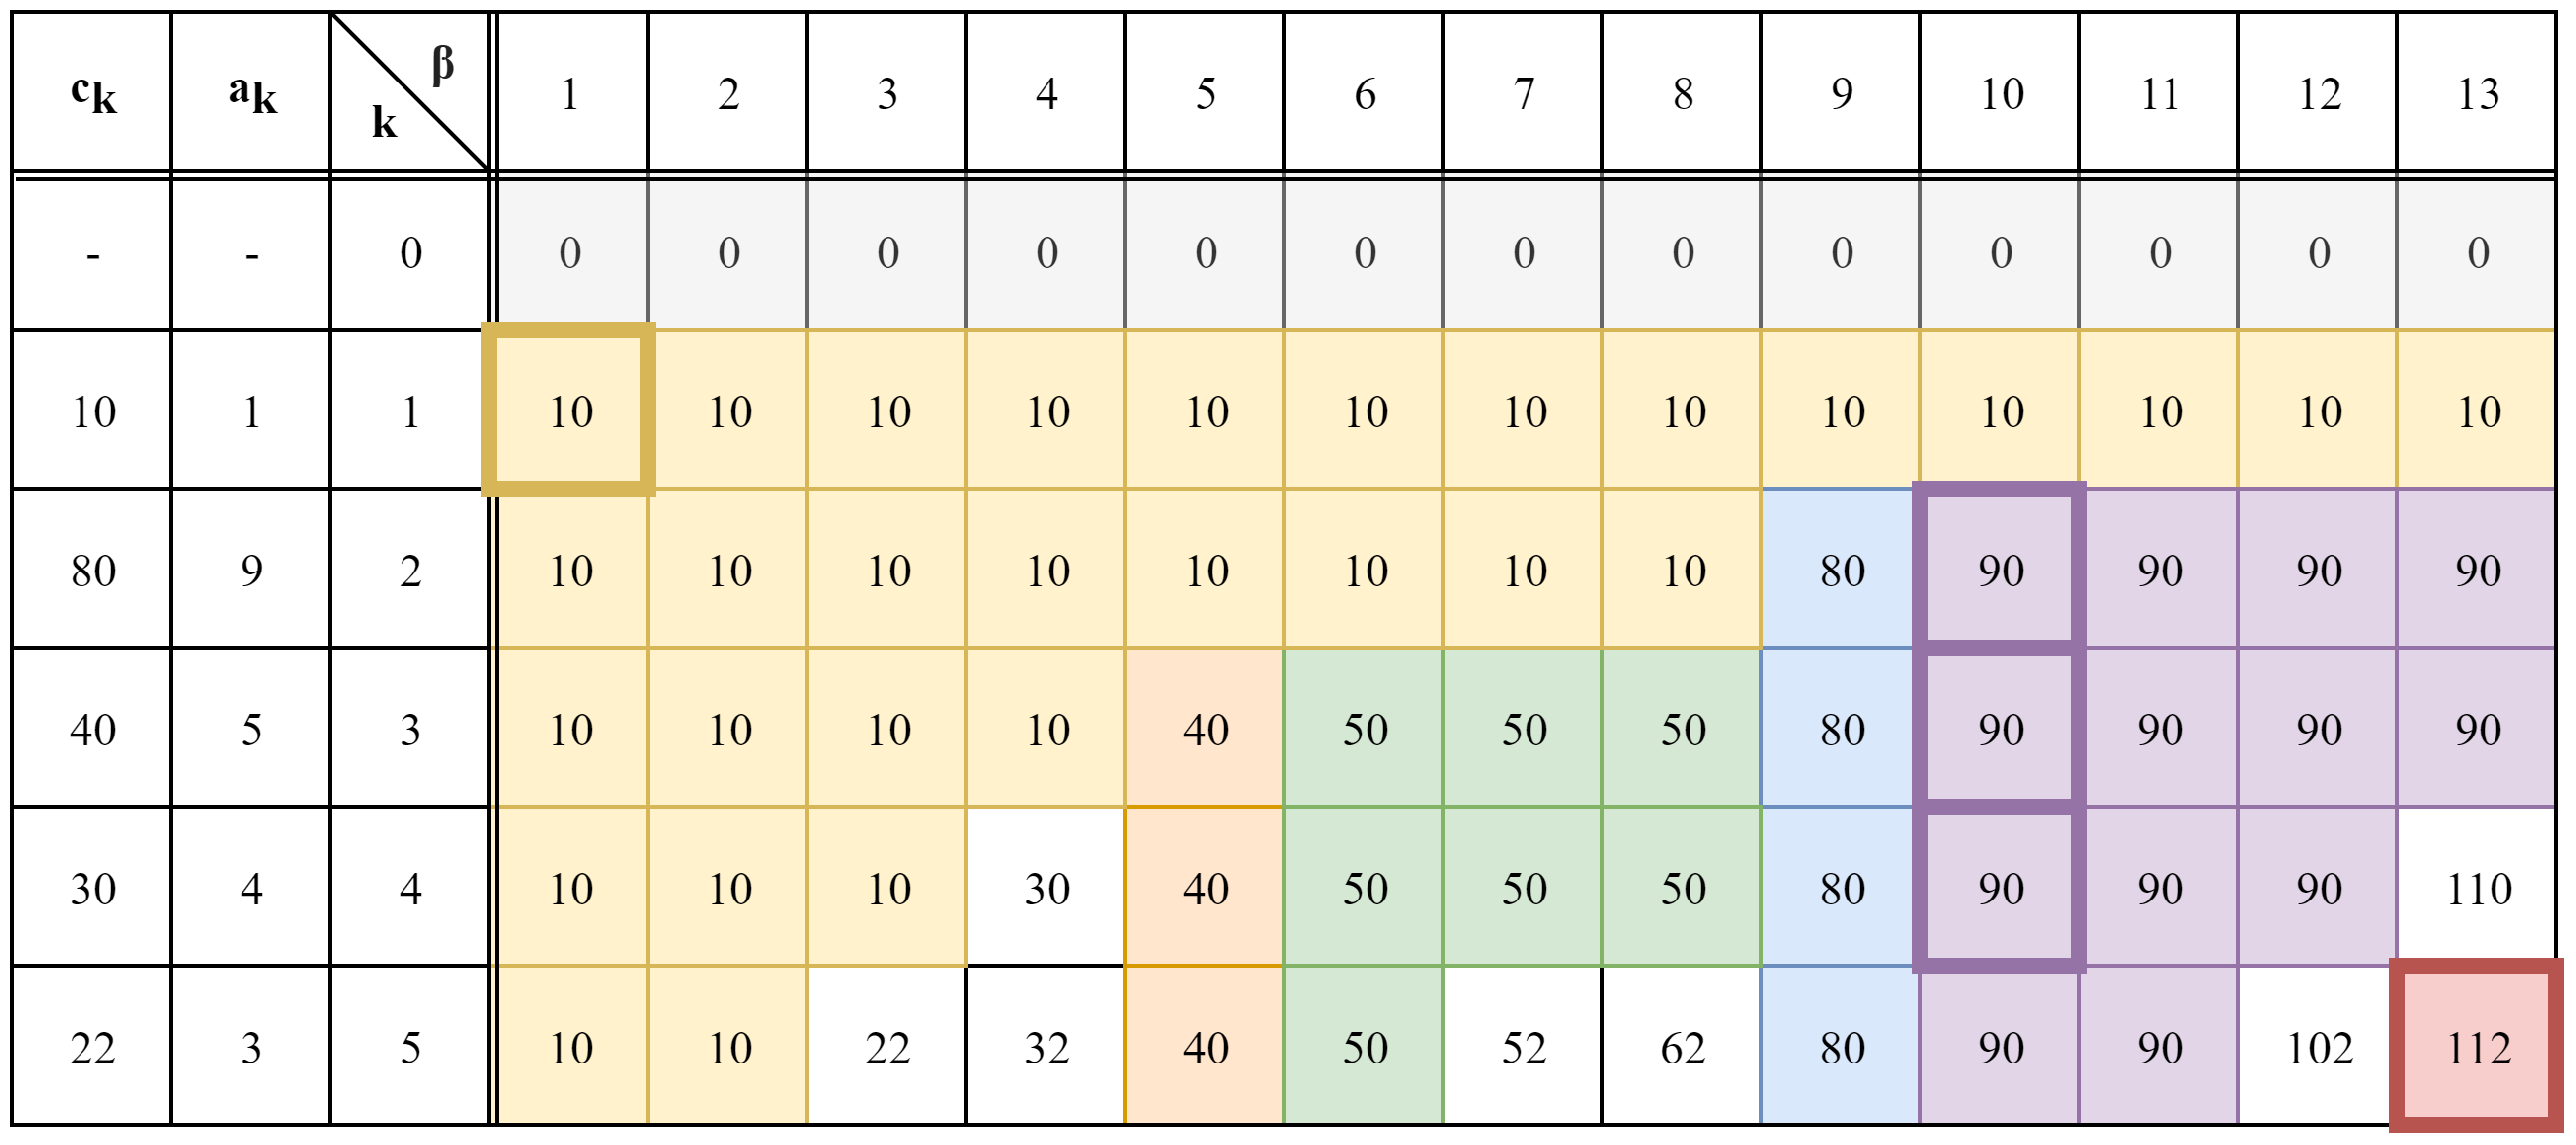
\includegraphics[width=0.95\linewidth,keepaspectratio]{KSP.png}
    \end{center}
    

\section{ Flüsse in Netzwerken }
    Ein (Fluss-)Netzwerk $N = (D,c,s,t)$ ist ein Digraph $D = (V,A)$ mit einer Kapazitätsfunktion $c: A \mapsto \mathbb{R}_+$ und zwei ausgezeichneten 
    Knoten $s$, genannt Quelle, und $t$, genannt Senke. $N$ simuliert einen Fluss $f: A \mapsto \mathbb{R}_+$ (Wasser, Elektrizität, Verkehr, etc.) 
    von der Quelle $s$ zur Senke $t$.

    \subsection*{ Kapazitätsbedingung }
    Für alle Kanten aus $A$ gilt: der Fluss $f(e)$ über eine Kante $e \in A$ ist nach oben beschränkt durch die Kapazität $c(e)$ der Kante.
    
    \subsection*{ Flusserhaltungsbedingung }
    Für alle Knoten aus $V$ außer $s$ und $t$ gilt: die Summe des Zuflusses eines Knotens $v \in V$ (Summe der Flüsse aller in $v$ eingehenden Kanten) muss gleich der Summe aller 
    Ausflüsse (Summer der Flüsse aller aus $v$ ausgehenden Kanten) sein.

    \subsection*{ Gesamtfluss $|f|$ }
    Der Gesamtfluss $|f|$ ist die Differenz aller Ausflüsse und Einflüsse der Quelle $s$ (alternativ die Differenz aller Einflüsse und 
    Ausflüsse der Senke $t$).

    \subsection*{ s-t-Schnitt }
    Ein s-t-Schnitt ist eine Teilmenge $S$ der Knotenmenge $V$, sodass $S$ die Quelle $s$, nicht aber die Senke $t$ enthält.
    Die Kapazität des Schnitts ergibt sich aus der Summe der Kapazitäten aller Kanten, die aus $S$ herausragen - also Knoten aus $S$ 
    mit Knoten verbinden, die nicht in $S$ enthalten sind.

    \subsection*{ augmentierender Weg }
    Ein augmentierender Weg ist ein Weg von $s$ nach $t$, auf dem die Kapazität keiner Kante voll ausgeschöpft ist, also für jede im Weg enthaltene 
    Kante $e$ gilt $f(e) < c(e)$. Der Fluss entlang des Weges ist also noch nicht maximal und kann daher auf jeder Kante um die kleinste $c(e) - f(e)$ 
    Differenz des ganzen Weges erhöht werden.

    \subsection*{ Residualgraph $D_f$ }
    Der Residualgraph $D_f$ zu einem Netzwerk $N$ und einem Fluss $f$ beschreibt durch Vorwärts- und Rückwärtskanten, um wie viel der Fluss jeder Kante von $N$ 
    erhöht und erniedrigt werden kann, sodass die Kapazitäts- und Flussbedingung erhalten bleiben. Für jede Kante in $N$, auf der der Fluss um Wert $x$ erhöht 
    werden kann, wird in $D_f$ eine korrespondierende Vorwärtskante mit Gewicht $x$ eingetragen. Für jeden auf einer Kante in $N$ bereits existierenden Fluss mit Wert $y$ 
    wird eine korrespondierende Rückwärtskante mit Gewicht $y$ eingetrage (der Fluss kann hier um $y$ reduziert werden).
    
    \subsection{ Max-Flow-Min-Cut-Theorem }
    Ein s-t-Fluss in einem Netzwerk ist genau dann maximal, wenn es keinen augmentierenden Weg mehr gibt. Der Wert eines maximalen s-t-Flusses stimmt mit dem Wert 
    der minimalen Kapazität eines s-t-Schnitts überein.

    \subsection{ Edmonds-Karp }
    Der Algorithmus von Edmonds und Karp erschließt sich systematisch kürzeste augmentierende Wege durch Breitensuche (\verb|find_augmenting_path|) und erhöht dann den Fluss entlang dieser Wege so 
    weit wie möglich (\verb|augment_flow|). Wenn kein augmentierender Weg mehr gefunden werden kann, ist der Fluss maximal.

    \large
\begin{verbatim}
find_augmenting_path()
    \end{verbatim}
    \small
\begin{verbatim}
input:  ein Flussnetzwerk N,
        ein Fluss flow
output: ein augmentierender Weg gegeben über die Vorgänger-Beziehung,
        ein minimaler Wert, um den der Fluss entlang des augmentierenden 
        Weges erhöht werden kann,
        eine Orietierungsfunktion, die Knoten als über Vorwärts- oder 
        Rückwärtskanten erreichbar markiert,
        ein korrespondierender s-t-Schnitt

predecessor
flow_delta()
orientation()
cut

markiere s, indem s cut hinzugefügt wird
foreach( Knoten v )
    flow_delta(v) = infinity

führe von s Breitensuche aus mit:
    if( neuer Knoten w ist über Vorwärtskante erreichbar )
        orientation(w) = +
        flow_delta(w) = Minimum aus flow_delta(predecessor(w)) und Wert, 
                        um den der Zufluss von w erhöht werden kann
    else
        orientation(w) = -
        flow_delta(w) = Minimum aus flow_delta(predecessor(w)) und Zufluss 
                        von w
    predecessor(w) = v
    markiere w, indem w cut hinzugefügt wird

return (predecessor, flow_delta(t), orientation, cut)
    \end{verbatim}
\normalsize

    \large
\begin{verbatim}
augment_flow()
    \end{verbatim}
    \small
\begin{verbatim}
input:  ein Flussnetzwerk,
        ein Fluss flow,
        ein augmentierender Weg gegeben über eine Vorgänger-Beziehung 
        predecessor,
        ein minimaler Wert flow_delta, um den der Fluss entlang des 
        augmentierenden Weges erhöht werden kann,
        eine Orietierungsfunktion, die Knoten als über Vorwärts- oder 
        Rückwärtskanten erreichbar markiert
output: ein um flow_delta augmentierter Fluss

v = t
w = undefined

while( w ungleich s )
    w = predecessor(v)
    if( orientation(v) = + )
        flow(w,v) = flow(w,v) + flow_delta
    else
        flow(w,v) = flow(w,v) - flow_delta
    v = w
    \end{verbatim}
\normalsize

    \large
\begin{verbatim}
edmonds_karp()
    \end{verbatim}
    \small
    \begin{verbatim}
input:  ein Flussnetzwerk N
output: ein maximaler Fluss,
        ein minimaler Schnitt

flow()
cut

foreach( Kante e des Netzwerkes )
    flow(e) = 0
cut = alle Knoten des Netzwerkes

while( Senke ist noch in cut enthalten )
    (path, flow_delta, orientation, new_cut) = find_augmenting_path(N, flow)
    cut = new_cut
    if( Senke ist noch in cut enthalten )
        flow = augment_flow(flow, path, flow_delta, orientation)

return flow, cut
    \end{verbatim}
\normalsize

    \subsection{ Push-Relabel }
    Der Push-Relabel-Algorithmus erzeugt - im Gegensatz zum Algorithmus von Edmonds und Karp - nicht in jedem Schritt einen korrekten Fluss, sonder arbeitet mit 
    sogenannten Präflüssen, einem  \shorthandoff{"}"Arbeitsfluss"\shorthandon{"}, der noch zum maximalen Fluss ausgearbeitet werden muss. Im Präfluss darf der 
    Zufluss eines Knotens größer als sein Abfluss sein, jedoch darf der Präfluss die Kapazitätsgrenzen der Kanten nicht übersteigen. Der Überschuss, der in 
    einem Knoten $v$ durch einen höheren Zu- als Abfluss entstehen kann, wird Exzess $e(v)$ genannt. Ein Knoten, dessen Exzess größer $0$ ist, wird aktiv genannt. 
    Ein Präfluss ist genau dann ein gültiger Fluss, wenn es keine aktiven Knoten gibt.
    \newline
    Idee des Push-Relabel-Algorithmus ist, von der Quelle den größtmöglichen Präfluss ins Netzwerk ausströmen zu lassen und alle 
    (ungültigen) Exzesse zukzessive \shorthandoff{"}"zurückzuschieben"\shorthandon{"}, sodass ein maximaler gültiger Fluss entsteht. Damit nicht im Kreis 
    zurückgeschoben wird, werden Knoten, die einen Exzess ausgeglichen haben, angehoben auf eine Höhe $d$. Die Höhe der Senke $d(t)$ ist $0$.
    \newline
    Hierzu werden zu Beginn alle Abflüsse der Quelle auf deren Maxima (= Kapazitäten) und die Flüsse über alle anderen Kanten auf $0$ gesetzt - somit sind alle
    Nachbarn der Quelle aktiv. Zudem wird die Quelle auf die Höhe $d(s) = |V|$ Anzahl der Knoten im Netzwerk angehoben. Alle anderen Knoten haben Höhe $0$. Man 
    wählt nun sukzessive (z.B. nach lexikographischer Ordnung) einen aktiven Knoten $v$ aus bis es keinen aktiven Knoten mehr gibt und führt je eine der folgenden zwei Operationen aus:
    \paragraph*{Relabel}, wenn alle Nachbarn, auf die $v$ schieben kann, höher als $v$ selbst liegen.
    \paragraph*{Push}, wenn zumindest ein Nachbarn, auf den $v$ schieben kann, mindestens ein Level niedriger liegt.
    \newline
    \verb|Relabel(v)|: hebe $v$ ein Level höher als den niedrigsten all seiner höheren beschiebbaren Nachbarn.
    \newline
    \verb|Push(v,w)|: $\gamma = $ Minimum aus Exzess $e(v)$ und schiebbarem Betrag zum niedrigsten Nachbarn $w$ aller niedrigeren beschiebbaren Nachbarn von $v$. 
    Schiebe $\gamma$-viel von $v$ auf $w$ und passe den Exzess von $v$ und die Restkapazität der Kante $(v,w)$ entsprechend an. 

\section{ Matchings }
    \subsection*{ Matching $M$ }
    In einem Graphen $G = (V,E)$ nennt man eine Kantenteilmenge $M \subseteq E$ Matching, wenn keine zwei Kanten aus $M$ einen gemeinsamen Endknoten haben. 
    Ist ein Knoten $v$ Endpunkt einer in $M$ enthaltenen Kante, nennt man $v$ $M$-gesättigt, ansonsten $M$-ungesättigt oder exponiert. 
    \newline
    Ein Matching $M$ heißt perfekt, wenn jeder Knoten in $G$ $M$-gesättigt ist. 
    \newline
    Ein Matching $M$ heißt maximal, wenn es kein Matching $M'$ in $G$ gibt, das mehr Kanten enthält als $M$.
    \subsection*{ Alternierender Pfad $P$ }
    In einem Graphen $G = (V,E)$, der ein Matching $M$ enthält, ist ein alternierender Pfad ein Pfad, der nur aus Kanten besteht, die abwechselnd zu $M$ und 
    den Rest-Kanten $E \setminus M$ gehören. Ist in einem alternierenden Pfad der erste und der Letzte Knoten $M$-ungesättigt (hierzu muss der Pfad gerade Länge haben), 
    nennt man den Pfad $M$-erweiternd oder $M$-augemntierend. Tauscht man in einem $M$-augmentierenden Pfad alle Kanten (flip) so, dass genau die Kanten zum 
    Matching gehören, die davor zu den Rest-Kanten gezählt haben, und umgekehrt, erhält man einen alternierenden Pfad, dessen Enden gesättigt sind - man hat 
    das Matching um die beiden vormals ungesättigten Endknoten des Pfades erweitert:
    \[ 1-2=3-4=5-6 \quad \rightarrow \quad 1=2-3=4-5=6 \]
    \newline
    Ein Matching $M$ ist genau dann maximal, wenn es keinen $M$-augmentierenden Pfad mehr gibt.
    \subsection*{ Symmetrische Differenz }
    Seien $M_1$ und $M_2$ Matchings im Graphen $G = (V,E)$, dann ist die symmetrische Differenz von zwei Matchings definiert als:
    \[ M_1 \triangle M_2 = (M_1 \setminus M_2) \cup (M_2 \setminus M_1) \]
    Für jede Zusammenhangskomponente $K$ des Untergraphen $G_{\triangle} = (V,M_1 \triangle M_2)$ von $G$ gilt eine der folgenden 
    Eigenschaften:
    \begin{itemize}
        \item $K$ ist ein Zyklus gerader länge mit Kanten abwechselnd in $M_1$ und $M_2$.
        \item $K$ ist ein Weg , dessen Kanten abwechselnd in $M_1$ und $M_2$ liegen und dessen Endknoten in einem der beiden Matchings ungesättigt sind.
    \end{itemize}
    \subsection*{ Heiratssatz von Hall }
    In einem bipartiten Graphen $G = (V = V_1 \uplus V_2, E)$ mit Bipartition $V_1$/$V_2$ gibt es genau dann ein matching, dass jeden Knoten in $V_1$ sättigt, 
    wenn für jede Teilmenge $U \subseteq V_1$ für die Menge der mit einem Element aus $U$ adjazenten Knoten $N(U)$ gilt:
    \[ |U| \leq |N(U)| \]

    \subsection*{ Blossom-Shrinking }
    Der Blossom-Shrinking-Algorithmus findet ein maximales Matching $M$ in einem Graphen $G=(V,E)$. Hierzu findet er durch Breitensuche $M$-augmentierende Pfade 
    und tauscht (flip) deren Kanten wie oben beschrieben, um $M$ um die Endknoten des jeweiligen Pfades zu erweitern.
    \newline
    Die Breitensuche startet immer vom lexikographisch kleinsten exponierten Knoten. Der entstehende Breitensuchbaum ist ein alternierender Baum, 
    dessen Kantenebenen abwechselnd nur Matching-Kanten oder nur Rest-Kanten enthalten.
    \newline
    Wird ein ungerader Kreis, erkennbar als Nicht-Matching-Querkante oder -Rückwärtskante im alternierenden Baum, gefunden, liegt ein sogenanntes Blossom vor. Ein Blossom wird durch einen 
    neuen Knoten $v_*$ (lexikographisch $1$ größer als der bisherige lexikographisch größte Knoten) ersetzt. $v_*$ erhält alle in das Blossom eingehenden Kanten. 
    Hierbei können Dopplungen auftreten - in diesem Fall kann jeweils irgendeine der doppelten Kanten ausgewählt werden.
    \newline
    Ziel ist nun, erst den reduzierten Blossomknoten $v_*$ in eine maximale Matching-Verkantung einzubetten, dann das Innere des Blossoms auf die schon maximale
    umgebende Verkantung abzustimmen und ggf. letztere noch korrektiv anzupassen. Dazu führt man den bisherigen Prozess des Findens und Erweiterns augmentierender 
    Pfade fort, bis man einen Pfad findet, der den Knoten $v_*$ enthält, der das Blossom ersetzt hat. Je nach Einbindung von $v_*$ in den erweiterten Weg nach 
    dem Flip kann das Innere des Blossoms entsprechend auf einen längeren alternierenden Pfad angepasst werden, der dann das komplette Blossom enthält.
    \newline
    Kann kein weiterer augmentierender Pfad mehr gefunden werden, ist das Matching maximal und man ist fertig.

\section{ Euler- \& Hamiltonkreise }
    \subsection*{ Eulertour }
    Eine Eulertour in einem Graphen $G = (V,E)$ ist ein Pfad von einem Knoten $v$ zu einem Knoten $w$, der Jede Kante aus $E$ genau einmal enthält. 
    Ein zusammenhängender Graph besitzt genau dann eine Eulertour, wenn maximal zwei seiner Knoten ungeraden grad haben.
    \newline
    Ist die Eulertour geschlossen, spricht man von einem Eulerkreis. Besitzt ein Graph einen Eulerkreis, nennt man eulersch. Ein zusammenhängender Graph ist 
    genau dann eulersch, wenn der Grad jedes Knotens gerade ist.

    \subsection{ Chinesisches Postboten-Problem (CPP) }
    Gegeben ist ein Graph $G = (V,E)$ mit nichtnegativen Kantengewichten $c(e) \geq 0, \forall e \in E$. Ziel ist es, einen geschlossenen Pfad (Kreis) zu finden, 
    der jede Kante mindestens einmal durchläuft und dabei minimales Gesamtgewicht (Summe aller durchlaufenen Kantengewichte) hat (z.B. effiziente Route für 
    Postboten/Müllabfuhr im Straßennetz).
    \newline
    Ansatz: ein Eulerkreis ist die optimale Lösung, da er ja jede Kante genau einmal durchläuft.
    \begin{itemize}
        \item Ist der Grad aller Knoten von $G$ gerade, ist man fertig und muss nur noch eine Traversierung des Eulerkreises finden.
        \item Gibt es Knoten mit ungeradem Grad, so müssen Kanten doppelt abeglaufen werden. Um einen entsprechenden Eulerkreis konstruieren zu können, 
        muss der Grad der Knoten mit ungeradem Grad auf eine gerade Zahl angehoben werden. Dies geschieht durch Verdopplung der Kanten von Pfaden, die zwei Knoten mit 
        ungeradem Grad verbinden (dies ist möglich, da es immer eine gerade Anzahl von Knoten mit ungeradem Grad gibt - vgl. Handshaking-Lemma). Es gilt nun, alle 
        Knoten mit ungeradem Grad so zu verbinden, dass die entstehenden, verdoppelten Pfade aufsummiert das kleinste, zusätzlich Gewicht zum Graphen beisteuern.
    \end{itemize}

    \subsection*{ Hamiltonkreis }
    Ein Hamiltonkreis in einem Graphen $G = (V,E)$ mit mindestens 3 Knoten ist ein Kreis, der jeden Knoten aus $V$ genau einaml enthält. Besitzt ein Graph einen Hamiltonkreis nennt man ihn 
    hamiltonisch. Das Problem zu entscheiden, ob ein Graph einen Hamiltonkreis enthält, ist $NP$-vollständig.

    \subsection*{ Satz von Dirac }
    Ein Graph $G = (V,E)$ ist genau dann hamiltonisch, wenn für jeden Knoten $v$ aus $V$ gilt:
    \[ deg(v) \geq \lceil\frac{n}{2}\rceil, \quad \forall v \in V \]
    , wobei $n$ die Anzahl aller Knoten in $V$ beschreibt.

    \subsection{ Travelling-Salesman-Problem (TSP) }
    Gegeben ist der vollständige Graph $G = K_n$ mit nichtnegativen Kantengewichten $c(e) \geq 0, \forall e \in E$. Ziel ist es nun einen Hamiltonkreis mit 
    minimalem Gewicht zu finden (Handlungsreisender, der möglichst effizient alle Städte des Landes bereisen will). Wenn die Abstände (= Kantengewichte) die 
    Dreiecksungleichung ($c(u,w) \leq c(u,v) + c(v,w)$) erfüllen, nennt man das TSP metrisch. Das TSP ist $NP$-schwer. Daher sucht man 
    sogenannte Heuristiken - Verfahren, die zumindest eine Näherungslösung in polynomialer Zeit liefern.
    \subsubsection*{ Nearest-Neighbour-Heuristik }
    Starte an einem beliebigen Knoten und baue von dort aus den Pfad auf. Füge dem Pfad vom Startknoten ausgehend solange immer den am schnellsten erreichbaren 
    (noch nicht besuchten) Knoten hinzu, bis der Pfad alle Knoten enthält. Verbinde End und Anfang des Pfades.
    \subsubsection*{ Christofides-Heuristik }
    Die Christofides-Heuristik funtioniert nur für metrische TSPs.
    \begin{enumerate}
        \item Bestimme einen minimal aufspannenden Baum $S$ von $G$ (z.B. mit Kruskal).
        \item Sei $W$ die Menge der Knoten mit ungeradem Grad im Spannbaum $S$.
        \item Finde Pfade in $G$, die alle Knoten aus $W$ möglichst effizient verbinden.
        \item Der Graph $G_*$, der aus Kombination des Spannbaumes $S$ und der Kanten der Pfade, die die ungeraden Knoten verbinden, entsteht ist eulersch.
        \item Bestimme eine Eulertour.
        \item Verkürze die Eulertour (Dreiecksungleichung).
    \end{enumerate}


\section{ Färbung von Graphen }
    \subsection{ Färbung planarer Graphen }

    \subsection{ Heuristiken zur Graphenfärbung }


\end{multicols*}
\end{document}
